\documentclass[10pt]{article}
\usepackage{amsmath,amsfonts,bm}
\usepackage{amsmath}
\usepackage{amssymb}
\usepackage{tikz}
\usepackage{pgfplots}
\usepackage{xcolor}
\usetikzlibrary{shapes, positioning, fit, backgrounds, tikzmark}
\pgfplotsset{compat=newest}
\usepgfplotslibrary{fillbetween}
\usepackage{color-edits}

\begin{document}

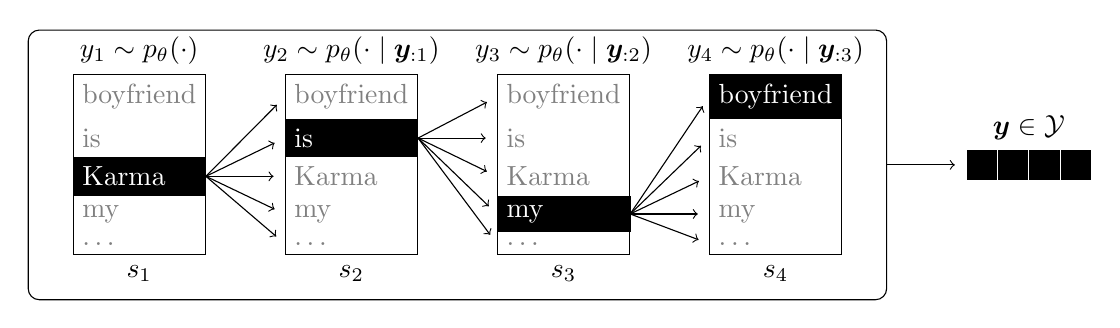
\begin{tikzpicture}[
    vocab/.style={
      draw,
      text=gray,
      rectangle split,
      rectangle split parts=5,
      rectangle split part align=left,
      rectangle split draw splits=false,
    }
  ]
  \node[
    vocab,
    rectangle split part fill={none, none, black, none},
    label=below:\(s_1\),
    label=above:\(y_1\sim p_\theta(\cdot)\),
  ] (s1)  {
    \nodepart{one} {boyfriend}
    \nodepart{two} {is}
    \nodepart{three} \textcolor{white}{Karma}
    \nodepart{four} {my}
    \nodepart{five} {\ldots}
  };
  \node[
    vocab,
    rectangle split part fill={none, black, none},
    label=below:\(s_2\),
    label=above:\(y_2\sim p_\theta(\cdot\mid\boldsymbol{y}_{:1})\),
  ] (s2) [right=of s1] {
    \nodepart{one} {boyfriend}
    \nodepart{two} \textcolor{white}{is}
    \nodepart{three} {Karma}
    \nodepart{four} {my}
    \nodepart{five} {\ldots}
  };
  \foreach \part in {text west, two west, three west, four west, five west} {
    \draw[->, shorten >= 4pt] (s1.three east) -- (s2.\part);
  }
  \node[
    vocab,
    rectangle split part fill={none, none, none, black, none},
    label=below:\(s_3\),
    label=above:\(y_3\sim p_\theta(\cdot\mid\boldsymbol{y}_{:2})\),
  ] (s3) [right=of s2] {
    \nodepart{one} {boyfriend}
    \nodepart{two} {is}
    \nodepart{three} {Karma}
    \nodepart{four} \textcolor{white}{my}
    \nodepart{five} {\ldots}
  };
  \foreach \part in {text west, two west, three west, four west, five west} {
    \draw[->, shorten >= 4pt] (s2.two east) -- (s3.\part);
  }
  \node[
    vocab,
    rectangle split part fill={black, none},
    label=below:\(s_4\),
    label=above:\(y_4\sim p_\theta(\cdot\mid\boldsymbol{y}_{:3})\),
  ] (s4) [right=of s3] {
    \nodepart{one} \textcolor{white}{boyfriend}
    \nodepart{two} {is}
    \nodepart{three} {Karma}
    \nodepart{four} {my}
    \nodepart{five} {\ldots}
  };
  \foreach \part in {text west, two west, three west, four west, five west} {
    \draw[->, shorten >= 4pt] (s3.four east) -- (s4.\part);
  }
  \node[draw, fit=(s1) (s2) (s3) (s4), inner sep=16pt, rounded corners] (decoding) {};
  \node[
    draw=white,
    rectangle split,
    rectangle split horizontal,
    rectangle split parts=4,
    rectangle split part fill=black,
    label=\(\boldsymbol{y}\in\mathcal{Y}\),
  ] (seq) [right=of decoding] {};
  \draw[->, shorten >= 4pt] (decoding) -- (seq);
\end{tikzpicture}

\end{document}